% !TEX encoding = UTF-8 Unicode

\documentclass[a4paper]{article}

\usepackage{xcolor}
\usepackage{url}
\usepackage[T2A]{fontenc} % enable Cyrillic fonts
\usepackage[utf8]{inputenc} % make weird characters work
\usepackage[margin=1in]{geometry}
\usepackage[serbianc]{babel}
\usepackage{CJKutf8}
\usepackage{graphicx}
\usepackage{fancyhdr}
\usepackage{listings}
\usepackage{csvsimple}
\usepackage{pgfplotstable}
\usepackage{longtable}
\usepackage{float}
\usepackage{amssymb}
\usepackage{amsthm}
\usepackage{mathtools}
\newtheorem{example}{Пример}
\newtheorem{lemma}{Лема}
\newtheorem{theorem}{Теорема}
\newtheorem{definition}{Дефиниција}
\newtheorem{property}{Својство}
\DeclareMathOperator{\mex}{mex}
% set the default code style

\definecolor{ghostwhite}{rgb}{0.98, 0.98, 0.98}
\definecolor{mediumviolet-red}{rgb}{0.78, 0.08, 0.52}
\definecolor{hooker\'sgreen}{rgb}{0.0, 0.44, 0.0}
\def\lstlistingname{Код}%
\lstset{
	language=C++,
	breaklines=true,
	backgroundcolor=\color{ghostwhite},
	frame=tb, % draw a frame at the top and bottom of the code block
	tabsize=2, % tab space width
	showstringspaces=false, % don't mark spaces in strings
	numbers=left, % display line numbers on the left
	numberstyle=\color{gray},
	rulecolor=\color{black},
	keywordstyle=\color{mediumviolet-red}, % keyword color
	commentstyle=\color{hooker\'sgreen} %comment color
}
%\usepackage[english,serbianc]{babel} %ukljuciti babel sa ovim opcijama, umesto gornjim, ukoliko se koristi cirilica

\usepackage[unicode]{hyperref}
\hypersetup{colorlinks,citecolor=green,filecolor=green,linkcolor=blue,urlcolor=blue}

\pagestyle{fancy}
\fancyhf{}
\renewcommand{\headrulewidth}{0pt}
\fancyfoot[R]{\thepage}

\graphicspath{{./src/statistics/picture/}}

\begin{document}
\begin{titlepage}
    \begin{center}
        \vspace{0.5cm}
        
        \Large{
	        Универзитет у Београду\\
	        Математички факултет\\
        }
    
        \vspace{0.5cm}
        \Large{Мастер рад}    
        
        \vspace{2.0cm}
        
        \Huge
        \rule[0.5cm]{\textwidth}{0.5pt}
        \textbf{Игра ним}
        \rule{\textwidth}{0.5pt}
        \vspace{0.5cm}
        
        \vspace{2.0cm}
        
        \begin{minipage}[t]{0.47\textwidth}
        	\textnormal{\large{\bf Аутор:\\}}
        	{\large Марија Мијаиловић}
        \end{minipage}\hfill\begin{minipage}[t]{0.47\textwidth}\raggedleft
        	\textnormal{\large{\bf Ментор:\\}}
        	{\large Др Миодраг Живковић}
        \end{minipage}
        
        \vfill
        
        {\Large Катедра за рачунарство и информатику}
        
        \vspace{0.8cm}
        
        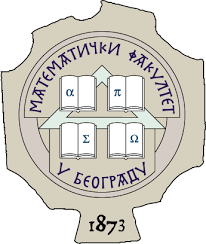
\includegraphics[width=0.3\textwidth]{matf_logo.png}
        
        \large{Београд, мај 2020}
        
    \end{center}
\end{titlepage}
\newpage
\pagenumbering{roman}
\tableofcontents

\newpage
\pagenumbering{arabic}
\section{Увод}
\label{sec:uvod}

\section{Ним}
\label{sec:nim}

Традиционална ним игра се игра у два играча са било којим предметима(новчићи, жетони, шибице, карте, ...), груписаних у гомиле. Број предмета и гомила је произвољан, тачније одређују их сами играчи. Играч који је на потезу може узети произвољан број жетона са једне гомиле, при чему мора узети бар један жетон и не сме узимати жетоне са више гомила. Играчи наизменично играју потезе. Како постоје нормалан и мизерни ним тип игре, постоје различити начини на које играч може да победи. У нормалном ниму побеђује играч који узме последњи жетон, док у мизерном губи играч који узме последњи жетон.

\begin{example}
На почетку партије на столу су три гомиле, са три, четири и пет жетона респективно. Партију играју два играча \textit{А} и \textit{Б}, \textit{А} игра први. 
\end{example}

Могући ток игре нормалног нима је приказан на слици \ref{fig:nimPrimer}.

\begin{figure}[H]
	\caption{Ток игре ним}
	\label{fig:nimPrimer}
	\begin{center}
		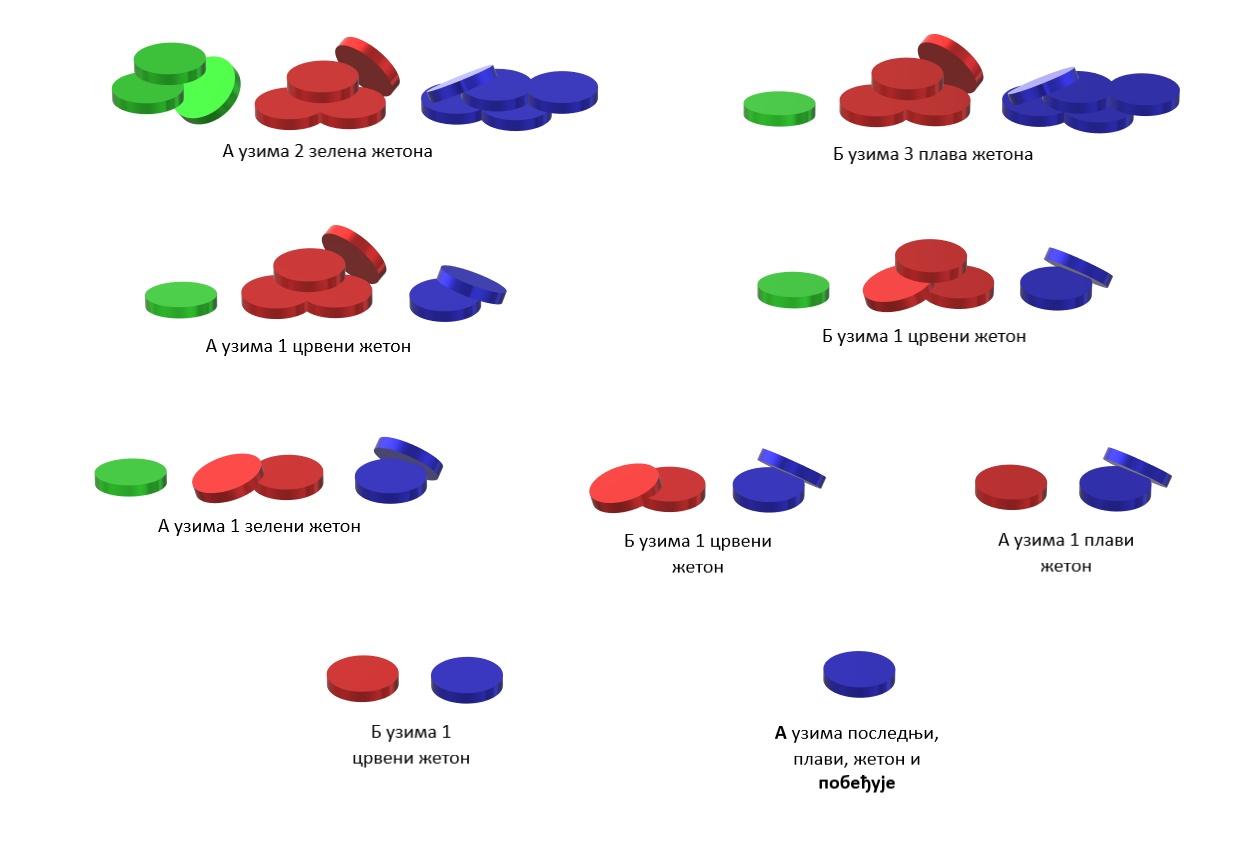
\includegraphics[width=\textwidth]{NimPrimer.png}
	\end{center}
\end{figure}

У општем случају, уколико се на столу налазе две гомиле, у зависности од броја жетона могући су следећи исходи нормалног нима:

\begin{itemize}
	\item Дате су две гомиле са по једним жетоном. Први играч мора да узме бар један жетон, чиме оставља другом играчу да узме последњи жетон и победи. У овој ситуацији очигледно је да \textbf{први играч загарантовано губи}.
	
	\item Дате су две гомиле, на првој један жетон, на другој два жетона. \textbf{Први играч има стратегију за победу}, уколико узме један жетон са гомиле где су два жетона (на слици \ref{fig:nimPrimer} узима 1 плави жетон), оставља следећем играчу две гомиле са по жетоном, а из претходног примера видели смо да је то стање у коме играч који је на потезу губи.
	
	\item Дате су две гомиле са по два жетона. Прва могућност јесте да први играч узме све са једне гомиле, чиме други играч истим тим потезом, узимајући све жетоне са друге гомиле побеђује. Друга могућност је да први играч узме један жетон, тако да је следеће стање игре заправо стање из претходног примера, у коме играч који је на потезу може да победи. У овој ситуацији \textbf{први играч губи} уколико други играч зна како треба играти ним.
\end{itemize}

Сада би требало да је јасно да у овој игри нема среће, већ да се најбољи потез може направити само ако се предвиди редослед потеза који ће уследити. Очигледно је да постоји неки образац који ће нам за конкретан број жетона и гомила рећи начин игре који ће играча довести до победе. Амерички математичар Чарлс Бутон (енг. {~\em Charles Bouton}) је извршио комплетну математичку анализу игре и 1902. године је пронашао трик. \cite{10.2307/1967631}

\section{Витхофова игра}
\label{sec:vithofova_igra}

Постоје многе варијанте нима, које се од оригиналне верзије углавном разликују по томе што садрже бар једно додатно правило за игру. Једна таква верзија је Витхофова игра (енг.{~\em Wythoff's game})\cite{10.2307/2321643}.

Витхофова игра је математичка стратешка игра за два играча. На столу се налазе две гомиле жетона; играчи наизменично узимају жетоне са једне или обе гомиле. Приликом узимања жетона са обе гомилe, рецимо $ k (> 0) $ са једне и $ l (> 0) $ са друге, мора да буде испуњен услов $ |k - l| < a $, где је $ a $ задати позитиван број који се одређује пре почетка партије и не мења се у току саме партије. Игра се завршава када број жетона на талону буде нула, а онај играч који је уклонио последњи жетон или жетоне је победник. Сваки играч када је на потезу мора да уклони бар један жетон.

У класичној Витхоф игри $ a $ je $ 1 $, што значи да ако играч узима жетоне са обе гомиле, број узетих жетона мора бити једнак.

Игра се еквивалентно може описати и као игра са краљицом на шаховској табли: имамо једну шаховску краљицу постављну било где на табли, сваки играч може да помера краљицу произвољан број корака у правцу југа, запада, или југозапада. Победник је играч који први помери краљицу у доњи леви угао табле.\cite{cut-the-knot, singingbanana-youtube}

Забележено је да се ова игра играла у Кини  под именом "\begin{CJK}{UTF8}{gbsn}捡石子\end{CJK} jiǎn shízǐ"(енг.{~\em picking stones}). \cite{Yaglom}

Холандски математичар В. А. Витхоф ({\em W. A. Wythoff}) је 1907. године објавио математичку анализу ове игре. \cite{wythoff1907modification}

\section{Оптимална стратегија}
\label{sec:optimalna_strategija}

Било која позиција се може представити паром бројева $ (x, y) $, где је $ x \le  y $, док  $ x $ и $ y $ представљају бројеве жетона на две гомиле или координате позиције краљице (при чему су координате доњег левог угла (0, 0)). Све могуће позиције могу се разврстати у две категорије, П-позиције и Н-позиције. 
\begin{definition}
	На П-позицји, играч који је на потезу губи ако противник игра како треба, другим речима наредни играч може да победи шта год одиграо противник. На Н-позицији, играч који је на потезу побеђује ако игра како треба.
\end{definition}

Класификација позиција на П и Н се дефинише рекурзивно на следећи начин:
\begin{enumerate}
	\item $ (0, 0) $ је П-позиција јер играч који је на потезу не може да одигра ниједан валидан потез, па је његов противник победник.
	\item Било која позиција са које је П-позиција достижна у једном потезу је Н-позиција. 
	\item Ако сваки потез води ка некој Н-позицији, онда је то П-позиција.
\end{enumerate}

Да би се Витхофова игра ирала на најбољи могући начин, потребно је знати две ствари:
\begin{itemize}
	\item Препознати природу тренутне позиције, да ли је П или Н.
	\item Уколико је тренутна позиција Н, треба израчунати следећи потез тако да се противник нађе у П позицији.
\end{itemize}

Разлог битности класификације на П и Н позиције лежи у чињеници да уколико је тренутна позиција Н, знамо да постоји потез који нас води на П-позицију, а тај потез можемо израчунати и победити. Са друге стране ако је тренутна позиција П не можемо урадити ништа, само одиграти произвољан валидан потез и надати се најбољем, с обзиром на то да се у једном потезу са П-позиције стиже на Н-позицију, са које противник може да победи ако зна да израчуна П-позицију. 

\begin{example}
	За $ a = 1 $, позиција $ (1, 2) $ је П-позиција, зато што су са ње у једном потезу достижне само позиције $ (0, 1), (0, 2), (1, 0) $ и $ (1, 1) $, које су Н-позиције. Још неке П-позиције приказане су у табели \ref{tab:a_1_Ppozicije}. 
\end{example}

\begin{table}[h!]
	\caption{Приказ првих $ 10 $ П-позиција за $ a = 1 $}
	\label{tab:a_1_Ppozicije}
	\begin{center}
		\begin{tabular}{  c | c | c }
			{\textbf{n}} &  {\textbf{A}} &  {\textbf{B}} \\
			\hline
			0 & 0 & 0 \\
			1 & 1 & 2 \\
			2 & 3 & 5 \\
			3 & 4 & 7 \\
			4 & 6 & 10 \\
			5 & 8 & 13 \\
			6 & 9 & 15 \\
			7 & 11 & 18 \\
			8 & 12 & 20 \\
			9 & 14 & 23 \\
			10 & 16 & 26\\ 
		\end{tabular}
	\end{center}
\end{table}

\begin{example}
	За $ a = 2 $, П-позиције приказане су у табели \ref{tab:a_2_Ppozicije}.
\end{example}

\begin{table}[h!]
	\caption{Приказ првих $ 10 $ П-позиција за $ a = 2 $}
	\label{tab:a_2_Ppozicije}
	\begin{center}
		\begin{tabular}{  c | c | c }
			{\textbf{n}} &  {\textbf{A}} &  {\textbf{B}} \\
			\hline
			0 & 0 & 0 \\
			1 & 1 & 3 \\
			2 & 2 & 6 \\
			3 & 4 & 10 \\
			4 & 5 & 13 \\
			5 & 7 & 17 \\
			6 & 8 & 20 \\
			7 & 9 & 23 \\
			8 & 11 & 27 \\
			9 & 12 & 30 \\
			10 & 14 & 34\\ 
		\end{tabular}
	\end{center}
\end{table}

\begin{example}
	На столу је табела $ 10x10 $, на позицији $ (0, 0) $ је циљ. Игру играју два играча \textit{А} и \textit{Б}, померајући наизменично краљицу од почетне позиције $ (x,y) $. Дозвољено је краљицу померати јужно, југозападно и западно у односу на текућу позицију.  Победник је играч који први доведе краљицу до циља.
\end{example}

Играч \textit{А} игра први, \textit{Б} други. На слици \ref{fig:sahovska_tabla_pozicije_a_2} је дат приказ П-позиција(зелена поља) и како се до њих може доћи(плаве и црвене стрелецие). Уколико је краљица на позицији $ (0, y), (x,0) $ или $ (x,x) $, при чему је $ x > 0, y > 0 $, играч \textit{А} уколико игра како треба у једном потезу може довести краљицу до циља и победити. Генерално, уколико је краљица на позицији, која одговара плавој или црвеној стрелици, играч \textit{А} може краљицу једним потезом довести до П-позиције, са које су достижне само Н-позиције и са којих играч \textit{А} може директно довести краљицу до циља или је померити на неку од преосталих П-позција ближих циљу. Уколико ниједна од плавих или црвених стрелица не одговара тренутној позицији краљице, играч који је на потезу уколико зна како на најбољи начин игратити Витхоф игру може победити. Решење у овом сучају нам дају рекурзивна, алгебарска или аритметичка стратегија, чији опис следи.
 
\begin{figure}[H]
	\caption{Приказ П-позиција на табли $ 10x10 $ за $ a = 2 $}
	\label{fig:sahovska_tabla_pozicije_a_2}
	\begin{center}
		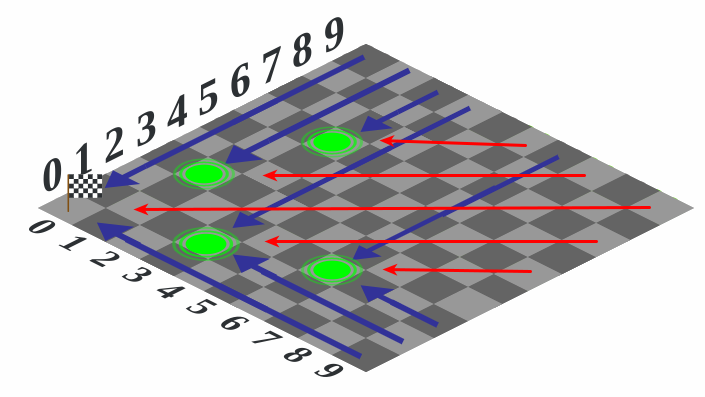
\includegraphics[width=\textwidth]{10x10_1.png}
	\end{center}
\end{figure}

\subsection{Рекурзивна стратегија}

\begin{definition}
	\label{def:mex}
	$\mex(A)$ означава најмањи природни број који није у скупу $ A $, тј. $ \mex(\emptyset)=0 $ и
$ \mex(A)=\min\{i | i\notin A\} $.
\end{definition}

Описани начин добијања П-позиција $ (A_{n}, B_{n}) $, може се поједноставити, што показује следећа теорема. 

\begin{theorem} [Рекурзивна карактеризација П-позиција]
	\label{thm:reukrzivna_strategija}
	Нека је 
	\begin{eqnarray}
		A_{n} = mex \{ A_{i}, B_{i} : i < n \} \\
		B_{n} = A_{n} + an 
	\end{eqnarray}
	Тада је скуп свих П-позиција
	$ P = \cup_{i=0}^{\infty} \{(A_{i},B_{i})\} $.
\end{theorem}

\begin{proof}
	
	Из дефиниција $ A_{n} $ и $ B_{n} $ датих у теореми важи да ако је $ A = \cup_{n=1}^{\infty} A_{n} $ и  $ B = \cup_{n=1}^{\infty} B_{n} $ онда су $ A_{n} $ и $ B_{n} $ \textbf{комплементарни} скупови, тако да $ A \cup B = Z^{+} $ је скуп целих позитивних бројева  и $ A \cap B = \emptyset $. Ово важи јер у случају да је $ A_{n} = B_{m} $, и $ n > m $, следи да је $ A_{n} $ $ \mex $ скупа који садржи $ B_{m} = A_{n} $ што је контрадикторно дефиницији \ref{def:mex}. Случај када је $ n \leq m $ је немогућ јер је тада $ B_{m} = A_{m} + am \geq  A_{n} + an > A_{n} $.
	
	Да би се доказала теорема довољно је показати да се из неке позиције $ (A_{n}, B_{n}) $ не може доћи у неку претходну позицију.
	
	У случају да се играч помера са $ (A_{n}, B_{n}) $ позиције, и узима само жетоне са једне гомиле, тим потезом производи позицију која није облика $ (A_{i}, B_{i}) $. Уколико узима жетоне са обе гомиле такође производи потез који није облика $ (A_{i}, B_{i}) $, у супротном уколико би произведена позиција била $ (A_{i}, B_{i}) $, морало би да важи $ |(B_{n} - B_{i}) - (A_{n}-A_{i})| < a $, ако искористимо да је $ B_{n} - A_{n} = an $ добијамо да треба да буде задовољено $ |(n-i)a| < a $, што је тачно само ако је $ i = n $, што је контрадикција. 
	
	У случају да се играч помера са позиције $ (x, y), x \le y $, позиција која није облика $ (A_{i}, B_{i}), i \ge 0 $. Како су $ A $ и $ B $ комплементарни скупови, може се сматрати да је $ x = B_{n} $, или је $ x = A_{n} $, за $ n \ge 0 $ .
	\begin{itemize}
		\item \label{case:slucaj1} Случај 1: $ x = B_{n} $ онда $ y = A_{n} $ 
		\item \label{case:slucaj2} Случај 2: $ x = A_{n} $, ако је $ y > B_{n} $ онда $ y = B_{n} $. Док у случају када је $ A_{n} \le y < B_{n} $ онда рачунамо $ d = y - x, m = \lfloor \frac{d}{a} \rfloor $ тако да је следећа позиција $ (A_{m}, B_{m}) $. Ово је легалан потез јер:
		\begin{enumerate}
			\item $ d = y - A_{n} < B_{n} - A_{n} = an $, стога $ m = \lfloor \frac{d}{a} \rfloor \le \frac{d}{a} < n $
			\item $ y = A_{n} + d \ge A_{m} + am = B_m $
			\item $ |(y - B_{m}) - (x - A_{m})| = |d - am| < a $
		\end{enumerate}
	\end{itemize}
	
\end{proof}

\subsection{Алгебарска стратегија}

\begin{definition}
	\label{def:alpha_beta}
	\begin{eqnarray}
		\alpha = \frac{2 - a + \sqrt{a^2 + 4}}{2} \\  
		\beta = \alpha + a
	\end{eqnarray}
	Где су $ \alpha $ и $ \beta $ ирационални за свако $ a > 0 $, и задовољавају $ \alpha^{-1} + \beta^{-1} = 1 $ .
\end{definition}

\begin{definition}
	\label{def:beati_niz}
	Нека је $ \alpha $ ирационалан позитиван број, тада је $ \lfloor \alpha n \rfloor $ Беати низ, где је $ n > 0 $.
\end{definition}

\begin{lemma}
	Нека су $ \alpha $ и $ \beta $ позитивни ирационални бројеви који задовољавају $ \alpha^{-1} + \beta^{-1} = 1 $ и нека је 
	\begin{eqnarray} 
		A_{n}^{'} = \lfloor \alpha n \rfloor\\
		B_{n}^{'} = \lfloor \beta n \rfloor\\
		A^{'} = \cup_{n=1}^{\infty}\{A_{n}^{'}\}\\
		B^{'} = \cup_{n=1}^{\infty}\{B_{n}^{'}\}
	\end{eqnarray}
	Тада су $ A^{'} $ и $ B^{'} $ комплементарни Беати низови.
\end{lemma}

\begin{proof}
	Довољно је показати да се тачно један елемент уније $ A_{n}^{'} \cup B_{n}^{'} $ налази у интервалу $ [N,N+1) $, за сваки позитиван број $ N $, тј. довољно је да одредимо колико има бројева из скупа $ A_{n}^{'} \cup B_{n}^{'} $ који су мањи од $ N $, ако је $ N > 1 $.
	
	Бројева из $ A_{n}^{'} $ мањих од $ N $ je $ \lfloor \frac{N}{\alpha} \rfloor $.
	
	Бројева из $ B_{n}^{'} $ мањих од $ N $ je $ \lfloor \frac{N}{\beta} \rfloor $.
	
	Важи:
		\begin{eqnarray}
			\frac{N}{\alpha} - 1 < \lfloor \frac{N}{\alpha} \rfloor < \frac{N}{\alpha} \label{eq:alpha}\\
			\frac{N}{\beta} - 1 < \lfloor \frac{N}{\beta} \rfloor < \frac{N}{\beta}
			\label{eq:beta}
		\end{eqnarray}
	
	Након сабирања (\ref{eq:alpha}) и (\ref{eq:beta}) добија се:
		\begin{displaymath}
		N - 2 < \lfloor \frac{N}{\alpha} \rfloor + \lfloor \frac{N}{\beta} \rfloor < N
		\end{displaymath} 
	Oдавде следи да је $ \lfloor \frac{N}{\alpha} \rfloor + \lfloor \frac{N}{\beta} \rfloor = N - 1 $, тј. $ N - 1 $ бројева из $ A_{n}^{'} \cup B_{n}^{'} $ је мање од $ N $. Слично важи и да је $ N $ бројева из $ A_{n}^{'} \cup B_{n}^{'} $ мање од $ N + 1 $. Тако да је $ N - (N - 1) = 1 $ елемент у интервалу $ [N,N+1) $ и нема дупликата.
\end{proof}

\begin{lemma}[Алгебарска карактеризација П-позиција] Нека су $ \alpha $ и $ \beta $ дефинисани као у \ref{def:alpha_beta}, тада је скуп свих П-позиција $ P = \cup_{n=0}^{\infty} \{(\lfloor \alpha n \rfloor, \lfloor \beta n \rfloor)\} $.
\end{lemma}

\begin{proof}
	Уочимо да је $ A'_{0} = 0, B'_{0} = 0 $ и $ B'_{n} - A'_{n} = an $. Такође како су $ A'_{n} $ и $ B'_{n} $ растући низови и комплементарни, важи још и да је $ A'_{n} = mex \{ A'_{i}, B'_{i} : i < n \} $. Што показује да је $ A'_{n} = A_{n} $ и $ B'_{n} = B_{n}  $ за $ n \ge 0 $.
	
	Нека је $ (x, y), x \leq y $ тренутна позиција игре, онда је $ x = \lfloor n \alpha \rfloor = A_{n} $, где је $ n = \lfloor \frac{(x+1)}{\alpha} \rfloor $ или је $ x = \lfloor n \beta \rfloor = B_{n} $, где је $ n = \lfloor \frac{(x+1)}{\beta} \rfloor $, даље се могу искористити Случај 1 и Случај 2 приказани у доказу теореме \ref{thm:reukrzivna_strategija}. Примера ради, ако је $ x = \lfloor n \alpha \rfloor = A_{n} $, и $ y < \lfloor n \beta \rfloor $ онда је $ m = \lfloor
	\frac{(y-x)}{a} \rfloor $ и следећа позиција је $ (\lfloor m \alpha \rfloor, \lfloor m \beta \rfloor) $ која је П-Позиција и није претходно посећивана.
\end{proof}

\begin{example}
	Специјални случај за $ a = 1 $ важи $ \alpha = \frac{1 + \sqrt{5}}{2} $ што је златни пресек.
	
	Низ $ \lfloor \alpha n \rfloor $ се назива доњи Витхофов низ ($ A_{n} $):
	$ 1, 3, 4, 6, 8, 9, 11, 12, 14, 16 $
	
	Низ $ \lfloor (\alpha + 1) n \rfloor $ се назива горњи Витхофов низ ($ B_{n} $):
	$ 2, 5, 7, 10, 13, 15, 18, 20, 23, 26 $
\end{example}

\subsection{Аритметичка стратегија}

\begin{definition}
	\label{def:verizni_razlomak}	
	Нека је $ \alpha $ ирационалан број, који задовоља $ 1 < \alpha < 2 $. Представља се једноставним бесконачним верижним разломком:
	
	\begin{eqnarray}
	\alpha = 1 + \frac{1}{a_{1} + \frac{1}{a_{2} + \frac{1}{a_{3} + ...}}} = [1, a_{1}, a_{2}, a_{3}, ...] 
	\end{eqnarray}
	
	где је $ a_{0}, a_{1}, ... $ јединствени бесконачни низ природних бројева за које важи $ a_{0} = 1 $ и $ a_{1}, a_{2}, ... ,  $ су позитивни и $ a_{n} \ne 1 $.
\end{definition}

\begin{definition}
	\label{def:p_q_nizovi}
	$ p $ и $ q $ су низови рекурзивно дефинисани на следећи начин:
	
	\begin{eqnarray}
		p_{-1} = 1, p_{0} = a_{0}, p_{n} = a_{n}p_{n-1} + p_{n-2}, (n \geq 1 )\\
		q_{-1} = 0, q_{0} = 1, q_{n} = a_{n}q_{n-1} + q_{n-2}, (n \geq 1 )
	\end{eqnarray}
	
	где је $ a_{0}, a_{1}, ... $ јединствени бесконачни низ природних бројева за које важи $ a_{0} = 1 $ и $ a_{1}, a_{2}, ... ,  $ су позитивни и $ a_{n} \ne 1 $.
\end{definition}

За $ \frac{p_{n}}{q_{n}} $ важи да је конвергент ирационалног броја $ \alpha $.  
\begin{displaymath}
	\frac{p_{n}}{q_{n}} = [1, a_{1}, , a_{2}, , a_{3}, ..., a_{n}]
\end{displaymath}

\begin{theorem}[Нумерације $ p $ и $ q $ система]
	\label{thm:p_q_sistemi}
	У $ p $-систему се сваки позитиван број јединствено може записати на следећи начин:
	
	\begin{eqnarray}
		N = \sum_{i=0}^{m} s_{i}p_{i}, 0 \le s_{i} \le a_{i+1}, s_{i+1} = a_{i+2} => s_{i}=0 , i \ge 0
	\end{eqnarray}
	
	слично важи и за $ q $-систем :
	
	\begin{eqnarray}
		N = \sum_{i=0}^{n} t_{i}q_{i}, 0 \le t_{0} \le a_{1}, 0 \le t_{i} \le a_{i+1}, t_{i} = a_{i+1} => t_{i-1}=0 , i \ge 1
	\end{eqnarray}
	
	где су $ p_{i} $ и $ q_{i} $ $ i $-ти елементи низова $ p $ и $ q $, дефинисаних \ref{def:p_q_nizovi}.
\end{theorem} 

\begin{proof}
	Дати број $ N $, где је $ m $ највећа вредност тако да је задовољено $ p_{m} \leq N $, може се записати:
	\begin{center}
		$ N = s_{m}p_{m} + r_{m}, 0 \leq r_{m} \le p_{m} $\\
		$ r_{m} = s_{m-1}p_{m-1} + r_{m-1}, 0 \leq r_{m-1} \le p_{m-1} $\\
		$ . $\\
		$ . $\\
		$ . $\\
		$ r_{i+1} = s_{i}p_{i} + r_{i}, 0 \leq r_{i} \le p_{i} $\\
		$ . $\\
		$ . $\\
		$ . $\\
		$ r_{1} = s_{1}p_{1} + r_{1}, 0 \leq r_{1} \le p_{1} $\\
		$ r_{0} = s_{0}p_{0} $
	\end{center}
	што одговара $ N = \sum_{i=0}^{m} s_{i}p_{i} $, где је $ s_{i}, i={0, ..., m} $ непознато и задовољава:
	\begin{displaymath}
		s_{i} = \frac{r_{i+1} - r_{i}}{p_{i}} < \frac{p_{i+1}}{p_{i}} = \frac{a_{i+1}p_{i}+p_{i-1}}{p_{i}} = a_{i+1} + \frac{p_{i-1}}{p_{i}} \leq a_{i+1} + 1 
	\end{displaymath}  
	тако да је $ 0 \leq s_{i} \leq a_{i+1}, i \geq 0 $.
\end{proof}

\begin{example}
	Приказ првих неколико бројева записаних у $ p $ и $ q $ систему, за $ a_{i} = 2 , i \ge 1 $ дат је у табели \ref{tab:p_q_sistem}.
\end{example}

\begin{table}[h!]
	\caption{Приказ првих неколико бројева записаних у $ p $ и $ q $ систему, за $ a_{i} = 2 , i \ge 1 $}
	\label{tab:p_q_sistem}
	\begin{center}
		\begin{tabular}{ | c | c | c | c | c  c | c | c | c | c | c |}
			\hline
			{$ \mathbf{q_{3}} $} &  {$ \mathbf{q_{2}} $} &  {$ \mathbf{q_{1}} $} &  {$ \mathbf{q_{0}} $} & & &  {$ \mathbf{p_{3}} $} &  {$ \mathbf{p_{2}} $} &  {$ \mathbf{p_{1}} $} &  {$ \mathbf{p_{0}} $} &\\
			12 & 5 & 2 & 1 & & & 17 & 7 & 3 & 1 &  {$ \mathbf{n} $}\\
			\hline
			&  &  & 1 & & &  &  &  & 1 & {$ \mathbf{1} $}\\
			&  & 1 & 0 & & &  &  &  & 2 & {$ \mathbf{2} $}\\
			&  & 1 & 1 & & &  &  & 1 & 0 &  {$ \mathbf{3} $}\\
			&  & 2 & 0 & & &  &  & 1 & 1 &  {$ \mathbf{4} $}\\
			& 1 & 0 & 0 & & &  &  & 1 & 2 &  {$ \mathbf{5} $}\\
			& 1 & 0 & 1 & & &  &  & 2 & 0 &  {$ \mathbf{6} $}\\
			& 1 & 1 & 0 & & &  & 1 & 0 & 0 &  {$ \mathbf{7} $}\\
			& 1 & 1 & 1 & & &  & 1 & 0 & 1 &  {$ \mathbf{8} $}\\
			& 1 & 2 & 0 & & &  & 1 & 0 & 2 &  {$ \mathbf{9} $}\\
			& 2 & 0 & 0 & & &  & 1 & 1 & 0 &  {$ \mathbf{10} $}\\
			& 2 & 0 & 1 & & &  & 1 & 1 & 1 &  {$ \mathbf{11} $}\\
			 1 & 0 & 0 & 0 & & & & 1 & 1 & 2 &  {$ \mathbf{12} $}\\
			 1 & 0 & 0 & 1 & & & & 1 & 2 & 0 &  {$ \mathbf{13} $}\\
			 1 & 0 & 1 & 0 & & & & 2 & 0 & 0 &  {$ \mathbf{14} $}\\
			 1 & 0 & 1 & 1 & & & & 2 & 0 & 1 &  {$ \mathbf{15} $}\\
			 1 & 0 & 2 & 0 & & & & 2 & 0 & 2 &  {$ \mathbf{16} $}\\
			 1 & 1 & 0 & 0 & & & 1 & 0 & 0 & 0 &  {$ \mathbf{17} $}\\
			\hline 
		\end{tabular}
	\end{center}
\end{table}

\begin{definition}
	Репрезентација $ R $ је  $ (m+1) $-торка за коју важи :
	\begin{eqnarray}
		R = (d_{m}, d_{m-1}, ... , d_{1}, d_{0}), 0 \le d_{i} \le a_{i+1}, d_{i+1} = a_{i+2} => d_{i} = 0, i \ge 0.
	\end{eqnarray}
\end{definition}

Уколико у $ R $ померимо сваку цифру $ d_{i} $ у лево за једно место добијамо $ R' = (d_{m}, d_{m-1}, ... , d_{1}, d_{0}, 0) $, а уколико је $ R $ репрезентација са $ d_{0} = 0 $ онда када сваку цифру $ d_{i} $ померимо за једно место у десно добијамо $ R'' = (d_{m}, d_{m-1}, ... , d_{1}) $ 

$ I_{p} = \sum_{i=0}^{m} d_{i}p_{i} $ je \textit{$ p $-интерпретација} репрезентације $ R $.

$ I_{q} = \sum_{i=0}^{m} d_{i}q_{i} $ je \textit{$ q $-интерпретација} репрезентације $ R $.

Може се приказати веза између $ p $-интерпретације и $ q $-репрезентације за позитиван број $ k $ :
\begin{eqnarray}
	I_{p}(R_{q}(k)) = I_{p}(d_{m}, d_{m-1}, ..., d_{1}) = n
\end{eqnarray} 

\begin{example}
	Број $ R_{q}(12) = 1000 $, а $ I_{p}(1000) = 17 $, ове вредности су приказане у табели \ref{tab:p_q_sistem}.
\end{example}

Описани $ p $ и $ q $ системи нумерације могу се искористити за још један начин добијања П-позиција, користећи следећа својства.

\begin{property}
	\label{prop:r_p_nule}
	Нека је $ n $ позитиван број. Уколико се $ R_p(n) $ репрезентација завршава парним бројем нула она је идентична вредности из скупа $ A_{n} $, а она $ R_p(n) $ репрезентација која се завршава непарним бројем нула идентичана је вредности из скупа $ B_{n} $.
\end{property}

\begin{example}
	Нека је $ n = 3 $ тада је $ R_{p}(3) = 10 $, што одговара вредности $ B_{1} = 3 $, ове вредности су приказане у табели \ref{tab:a_2_Ppozicije} и \ref{tab:p_q_sistem}.
\end{example}

\begin{example}
	Нека је $ n = 7 $ тада је $ R_{p}(7) = 100 $, што одговара вредности $ A_{5} = 7 $, ове вредности су приказане у табели \ref{tab:a_2_Ppozicije} и \ref{tab:p_q_sistem}.
\end{example}

\begin{example}
	Нека је $ n = 9 $ тада је $ R_{p}(9) = 102 $, што одговара вредности $ A_{7} = 9 $, ове вредности су приказане у табели \ref{tab:a_2_Ppozicije} и \ref{tab:p_q_sistem}.
\end{example}

\begin{property}
	\label{prop:levi_pomeraj}
	За свако $ n \geq 1 $ $ p $ репрезентација од $ B_{n} $ одговара левом померају $ p $ репрезентације од  $ A_{n} $
		\begin{displaymath}
			R_{p} (B_{n}) = R_{p}^{'} (A_{n}) 
		\end{displaymath}
\end{property}

\begin{example}
	Нека је $ n = 3 $ тада је $ A_{3} = 4 $ и $ B_{3} = 10 $.
	\begin{center}
		$ R_{p}(B_{3}) = R_{p}(10) = 110; $ \\
		$ R_{p}(A_{3}) = R_{p}(4) = 11; $ \\
		$ R_{p}^{'}(A_{3}) = 110; $ 
	\end{center}
	Ове вредности су приказане у табели \ref{tab:a_2_Ppozicije} и \ref{tab:p_q_sistem}.
\end{example}

\begin{property}
	\label{prop:r_q_nule}
	Нека је $ n $ позитиван број. Уколико се $ R_q(n) $ репрезентација завршава парним бројем нула онда је :
	\begin{displaymath}
		I_{p}(R_q(n)) = A_{n}
	\end{displaymath}
	Уколико се $ R_q(n) $ репрезентација завршава непарним бројем нула: 
	\begin{displaymath}
		I_{p}(R_q(n)) = A_{n} + 1
	\end{displaymath}
\end{property}

\begin{example}
	Нека је $ n = 10 $, тада је $ I_{p}(R_q(10)) = I_{p}(200) = 14 = A_{10} $, ове вредности су приказане у табели \ref{tab:a_2_Ppozicije} и \ref{tab:p_q_sistem}.
\end{example}

\begin{example}
	Нека је $ n = 7 $, тада је $ I_{p}(R_q(7)) = I_{p}(110) = 10 = A_{7} + 1 $, ове вредности су приказане у табели \ref{tab:a_2_Ppozicije} и \ref{tab:p_q_sistem}.
\end{example}

На основу својстава \ref{prop:r_p_nule}, \ref{prop:levi_pomeraj} и \ref{prop:r_q_nule} може се извршити карактеризација текуће позиције и одредити следећи потез.

Претпоставимо да је текућа позиција $ (x, y), 0 < x \le y $, прво је потребно ирачунати $ R_{p}(x) $ и проверити да ли се завршава са парним или непарним бројем нула.

Уколико се завршава непарним бројем нула онда је $ x = B_{n} $, тако да је победнички потез $ (x, y) \rightarrow (I_{p}(R''_{p}(x)), x) $

Уколико се завршава парним бројем нула онда је $ x = A_{n} $, ако је $ y > I_{p}(R'_{p}(x)) $ победнички потез је $ (x, y) \rightarrow (x, I_{p}(R'_{p}(x)) $, иначе уколико је $ y < I_{p}(R'_{p}(x) $ рачунамо $ d = y - x, m = \lfloor \frac{d}{a} \rfloor $. Тако да уколико се сад $ R_{q}(m) $ завршава са парним бројем нула онда је $ A_{m} = I_{p}(R_{q}(m)) $, иначе уколико се завршава непарним бројем нула $ A_{m} = I_{p}(R_{q}(m)) - 1 $. У оба случаја победнички потез је $ (x, y) \rightarrow (A_{m}, A_{m} + ma) $

\section{Имплементација и евалуација}
\label{implementacija_evaluacija}

За сваку стратегију извршено је мерење конструкције П табеле, резултати извршавања у милисекундама зависно од $ n $, при фиксном $ a = 2 $ су приказани у табели \ref{tab:calculate_time_n}. 
За мерење је коришћена хроно библиотека (енг.{~\em chrono library}) \cite{chrono_library}. Сва мерења су извршена на раучунару са следећом конфигурацијом:
\begin{flushleft}
	CPU: Intel(R) Core(TM) i7-4510U CPU @ 2.00GHz\\
	RAM: Kingston 8GB 1600MHz DDR3\\
	OS: Debian GNU/Linux 9 (stretch)\\
	Compiler: gcc 6.3.0\\
\end{flushleft}

У табели \ref{tab:calculate_piles} приказане су величине парова жетона П табеле све до $ 10^{31} $, као и одговарајуће $ n $.

\subsection{Рекурзивна стратегија}

За раучунање П табеле рекурзивном стратегијом прво је потребно да израчунамо $ A_{i} $, тачније потребно је наћи $ mex $ (дефиниција (\ref{def:mex})). За тражење је коришћен помоћни низ димензије $ 2*n $, иницијализиван нулама. Тражење $ mex $-а  своди се на проналажење индекса прве нуле, с обзиром да за елементе $ A $ важи $ a <= 2*n $ сложеност у најгорем случају је $ O(n) $. Чиме је укупна временска сложеност конструкције П табеле $ O(n^2) $.\\

\lstinputlisting[language=C++, linerange={7-31}, caption=Рекурзивна стратегија рачунање П табеле]{./src/recursive.cpp}

\leavevmode\\
Графички приказ зависности $ n $ и времена у милисекундама дат је на слици \ref{fig:recursive}, за $ а = 2 $.

\begin{figure}[H]
	\caption{График рекурзивне стратегије за конструкцију П табеле}
	\label{fig:recursive}
	\begin{center}
		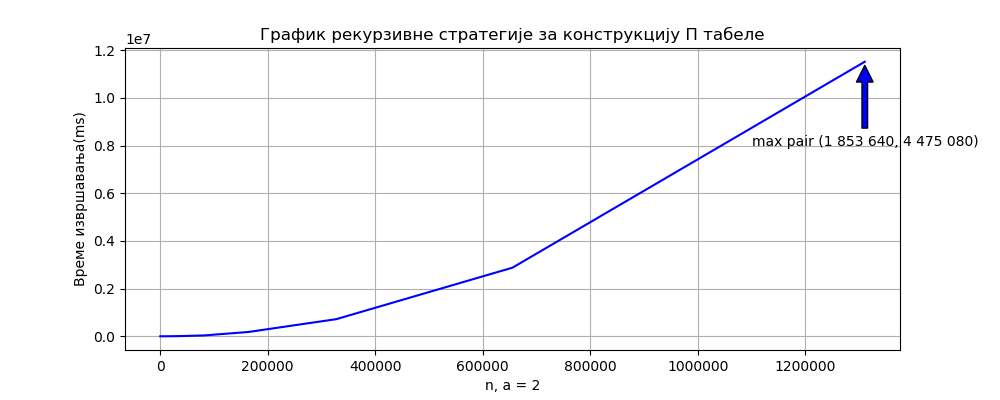
\includegraphics[width=\textwidth]{recursive.png}
	\end{center}
\end{figure}

\subsection{Алгебарска стратегија}

За разлику од рекурзиивне стратегије која користи имплицитну рекурзију, алгебарска стратегија користи експлицитну рекурзију, рачунајући $ alpha $ и $ beta $ (дефиниција (\ref{def:alpha_beta})). Чиме је укупна временска сложеност конструкције П табеле $ O(n) $.\\

\lstinputlisting[language=C++, linerange={10-24}, caption=Алгебарска стратегија рачунање П табеле]{./src/algebraic.cpp}

\leavevmode\\
Графички приказ зависности $ n $ и времена у милисекундама дат је на слици \ref{fig:algebraic}, за $ а = 2 $.

\begin{figure}[H]
	\caption{График алгебарске стратегије за конструкцију П табеле}
	\label{fig:algebraic}
	\begin{center}
		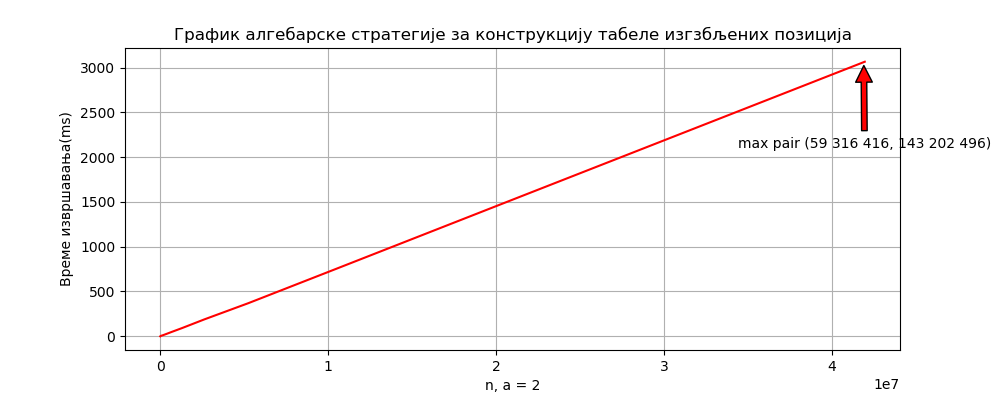
\includegraphics[width=\textwidth]{algebraic.png}
	\end{center}
\end{figure}

\subsection{Аритметичка стратегија}

За раучунање П табеле аритметичком стратегијом прво је потребно конструисати једноставан коначан верижни разломак, што захтева $ O(n) $ времена. 

Потом дефинишемо низове $ p $ и $ q $, њихова димензија је највише $ log(n) $, стога је врeме потребно да дефинишемо ове низове $ O(log(n)) $.

Преостаје још само да $ n $ бројева представимо у $ p $ и $ q $ систему, за њихово представљање у свакој итерацији имамо бинарну претрагу низова $ p $ и $ q $ којом се одређује са колико цифара треба представити број $ i $, што је у најгорем случају једнако величини низова $ p $ и $ q $, тачније $ log(n) $. Тако да је сложеност бинарне претраге $ O(log(log(n))) $. Репрезентација броја $ k $ у $ p $ или $ q $ систему се добија тако што рачунамо количник и остатак дељења броја $ k $ са одговарајућом вредности низа $ p $ или $ q $. Уколико имамо остатак потребно је и њега представити у $ p $ или $ q $ систему, његова $ p $ или $ q $ репрезентација је позната тако да је потребно само да је прекопирамо на крај текуће $ p $ или $ q $ репрезентације броја $ k $, не мењајући притом унапред дефинисан број цифара. Сложеност операције копирања једнака је броју елемената који се копира, што је у најгорем случају $ log(k) - 1 $ цифара. Како имамо $ n $ итерација укупна сложеност представљања првих $ n $ бројева у $ p $ и $ q $ систему захтева $ O(n(log(log(n)) + log(n) - 1)) $ времена.

Чиме је укупна временска сложеност конструкције П табеле $ O(nlog(n)) $

\lstinputlisting[language=C++, linerange={14-94}, caption=Аритметичка стратегија рачунање П табеле]{./src/arithmetic.cpp}

\leavevmode\\
Графички приказ зависности $ n $ и времена у милисекундама дат је на \ref{fig:arithmetic}, за $ a = 2 $.

\begin{figure}[H]
	\caption{График аритметичке стратегије за конструкцију П табеле}
	\label{fig:arithmetic}
	\begin{center}
		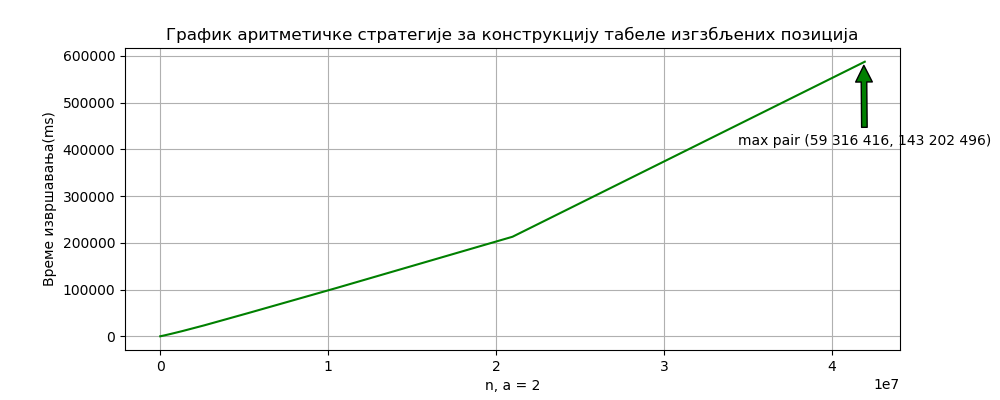
\includegraphics[width=\textwidth]{arithmetic.png}
	\end{center}
\end{figure}

\subsection{Сумиран приказ времена извршавања свих стратегија}

Из претходне анализе се може закључити да је алгебарска стратегија најефикаснија, што се може видети и на обједињеним графицима \ref{fig:all} и  \ref{fig:algebraicVSarithmetic}.

\begin{figure}[H]
	\caption{Сумиран приказ извршавања свих стратегија за конструкцију П табеле}
	\label{fig:all}
	\begin{center}
		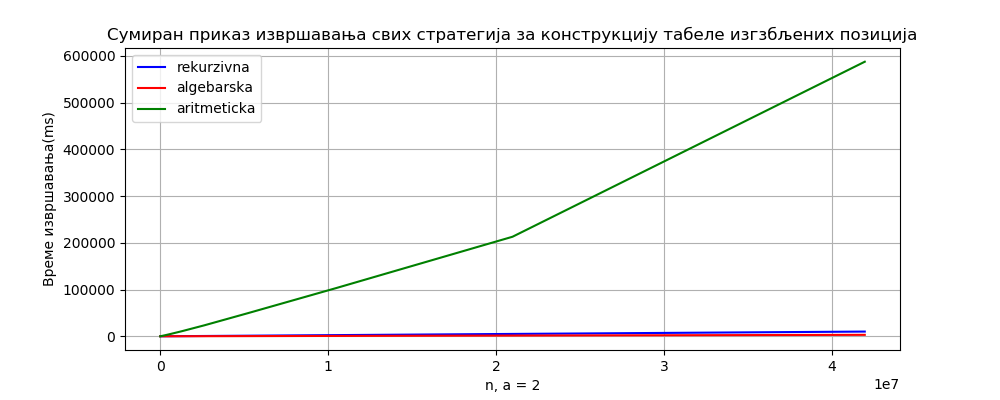
\includegraphics[width=\textwidth]{all.png}
	\end{center}
\end{figure}

\begin{figure}[H]
	\caption{Сумиран приказ извршавања алгебарске и аритметичке стратегије за конструкцију П табеле}
	\label{fig:algebraicVSarithmetic}
	\begin{center}
		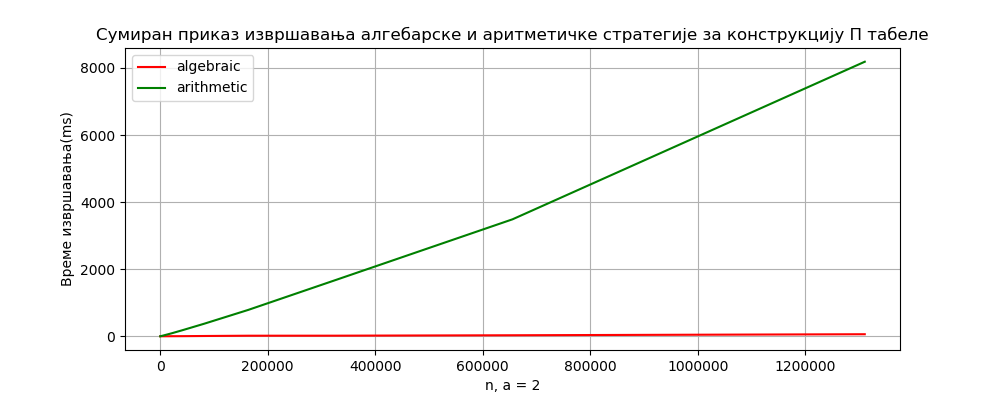
\includegraphics[width=\textwidth]{algebraicVSarithmetic.png}
	\end{center}
\end{figure}

\subsection{Препознавање природе тренутне позиције}

Када имамо израчунате П-позиције, можемо да анализирамо природу тренутне позиције и да одредимо следећу позицију игре.

На \ref{lst:recursive_and_algebraic}, приказан је код за рекурзивну и алгебарску стратегију којим се проверава да ли је текућа позиција П, и ако није одређује се следећа позиција тако да она буде П позиција.
За аритметичку стратегију, код је приказан на \ref{lst:arithmetic}.

\lstinputlisting[language=C++, linerange={30-58}, label={lst:recursive_and_algebraic}, caption= Достизање П позиције рекурзивном и алгебарском стратегијом]{./src/recursive_and_algebraic.cpp}

\lstinputlisting[language=C++, linerange={126-183}, label={lst:arithmetic}, caption= Достизање П позиције аритметичком стратегијом]{./src/arithmetic.cpp}

\newpage
\appendix
\section{Додатак резултатима}

\csvautolongtable[
table head=\caption{Времена извршавања у милисекундама конструкције П табеле}\label{tab:calculate_time_n}\\\hline
\csvlinetotablerow\\\hline
\endfirsthead\hline
\csvlinetotablerow\\\hline
\endhead\hline
\endfoot,
respect all
]{./src/statistics/csv/calculate_time_n.csv}

\csvautolongtable[
table head=\caption{Парови жетона П табеле}\label{tab:calculate_piles}\\\hline
\csvlinetotablerow\\\hline
\endfirsthead\hline
\csvlinetotablerow\\\hline
\endhead\hline
\endfoot,
respect all
]{./src/statistics/csv/calculate_piles.csv}

\newpage
\addcontentsline{toc}{section}{Литература}
\appendix
\bibliography{literatura} 
\bibliographystyle{plain}

\end{document}
